% !TeX spellcheck = en_US
% !TeX encoding = utf8
% !TeX program = xelatex
% !BIB program = bibtex

\documentclass[notes]{beamer}
% \documentclass[draft]{beamer}	
\usetheme{Singapore}
% \usecolortheme{default}
%\usepackage{pgfpages}
%\setbeameroption{show notes on second screen}

\usepackage[british]{babel}
\usepackage{graphicx,hyperref,url}
% \usepackage{ru}
\usepackage{mmstyles}
% \usepackage{hanging}
\usepackage{listings}
\usepackage{fontspec}
\usefonttheme[onlymath]{serif}
\usepackage{xeCJK}
% \usepackage[backend=biber]{biblatex}
% \bibliography{./ref.bib}
%\addbibresource{ref.bib}
\usepackage{indentfirst}
\usepackage{longtable}
\usepackage{float}
%\usepackage{picins}
\usepackage{rotating}
\usepackage{subfigure}
\usepackage{tabu}
\usepackage{amsmath}
\usepackage{amssymb}
\usepackage{setspace}
\usepackage{amsfonts}
\usepackage{appendix}
\usepackage{listings}
\usepackage{xcolor}
\usepackage{geometry}
% \setCJKfamilyfont{cjkhwxk}{SimSun}
% \newcommand*{\cjkhwxk}{\CJKfamily{cjkhwxk}}
%\newfontfamily{\consolas}{Consolas}
%\newfontfamily{\monaco}{Monaco}
%\setmonofont[Mapping={}]{Consolas}	%英文引号之类的正常显示,相当于设置英文字体
%\setsansfont{Consolas} %设置英文字体 Monaco, Consolas,  Fantasque Sans Mono
% \setmainfont{Times New Roman}
% \newfontfamily{\consolas}{Times New Roman}
% \newfontfamily{\monaco}{Arial}
% \setCJKmainfont{Times New Roman}
%\setmainfont{MONACO.TTF}
%\setsansfont{MONACO.TTF}
\newcommand{\verylarge}{\fontsize{60pt}{\baselineskip}\selectfont}  
\newcommand{\chuhao}{\fontsize{44.9pt}{\baselineskip}\selectfont}  
\newcommand{\xiaochu}{\fontsize{38.5pt}{\baselineskip}\selectfont}  
\newcommand{\yihao}{\fontsize{27.8pt}{\baselineskip}\selectfont}  
\newcommand{\xiaoyi}{\fontsize{25.7pt}{\baselineskip}\selectfont}  
\newcommand{\erhao}{\fontsize{23.5pt}{\baselineskip}\selectfont}  
\newcommand{\xiaoerhao}{\fontsize{19.3pt}{\baselineskip}\selectfont} 
\newcommand{\sihao}{\fontsize{14pt}{\baselineskip}\selectfont}      % 字号设置  
\newcommand{\xiaosihao}{\fontsize{12pt}{\baselineskip}\selectfont}  % 字号设置  
\newcommand{\wuhao}{\fontsize{10.5pt}{\baselineskip}\selectfont}    % 字号设置  
\newcommand{\xiaowuhao}{\fontsize{9pt}{\baselineskip}\selectfont}   % 字号设置  
\newcommand{\liuhao}{\fontsize{7.875pt}{\baselineskip}\selectfont}  % 字号设置  
\newcommand{\qihao}{\fontsize{5.25pt}{\baselineskip}\selectfont}    % 字号设置 

\graphicspath{{./fig/}}

% \setbeamertemplate{footnote}{%
%   \hangpara{2em}{1}%
%   \makebox[2em][l]{\insertfootnotemark}\footnotesize\insertfootnotetext\par%
% }

\definecolor{cred}{rgb}{0.6,0,0}
\definecolor{cgreen}{rgb}{0.25,0.5,0.35}
\definecolor{cpurple}{rgb}{0.5,0,0.35}
\definecolor{cdocblue}{rgb}{0.25,0.35,0.75}
\definecolor{cdark}{rgb}{0.95,1.0,1.0}
\lstset{
	language=R,
	numbers=left,
	numberstyle=\tiny\color{black},
	keywordstyle=\color{cpurple}\consolas,
	commentstyle=\color{cgreen}\consolas,
	stringstyle=\color{cred}\consolas,
	frame=single,
	escapeinside=``,
	xleftmargin=1em,
	xrightmargin=1em, 
	backgroundcolor=\color{cdark},
	aboveskip=1em,
	breaklines=true,
	tabsize=3
} 
% The title of the presentation:
%  - first a short version which is visible at the bottom of each slide;
%  - second the full title shown on the title slide;
\title[]{Fast Image Processing with Fully-Convolutional Networks}

% % Optional: a subtitle to be dispalyed on the title slide
% \subtitle{Optimization for Biosensor}

% % The author(s) of the presentation:
% %  - again first a short version to be displayed at the bottom;
% %  - next the full list of authors, which may include contact information;
\author[Zejia LV]{Zejia LV \\ zejialv@zju.edu.cn}
% % The institute:
% %  - to start the name of the university as displayed on the top of each slide
% %    this can be adjusted such that you can also create a Dutch version
% %  - next the institute information as displayed on the title slide

%\institute[IVLab, ZJU]{Data Science \& Engineering Research Center, ZJU}

% Add a date and possibly the name of the event to the slides
%  - again first a short version to be shown at the bottom of each slide
%  - second the full date and event name for the title slide
\date[\today]{\today}

\begin{document}

\AtBeginSection[]
{
	\begin{frame}
		\frametitle{Outline}
		\tableofcontents[currentsection]
	\end{frame}
}
\begin{frame}
	\titlepage
\end{frame}


\begin{frame}{Introduction}
	\begin{block}{Background}
	\begin{itemize}
		\item  	The computational demands and running times of existing operators vary greatly. 
		\item One general approach to accelerating a broad range of image processing operators is well-known: downsample the image, execute the operator at low resolution, and upsample. This can limit the accuracy of the approximation.
	\end{itemize}
	
	\end{block}	
	\begin{block}{What we do}
		Unlike the downsampling approach, the method operates on full resolution images, is trained end-to-end to maximize accuracy, and does not require running the original operator at all.
	\end{block}
\end{frame}

\begin{frame}{Introduction}
	\begin{figure}
			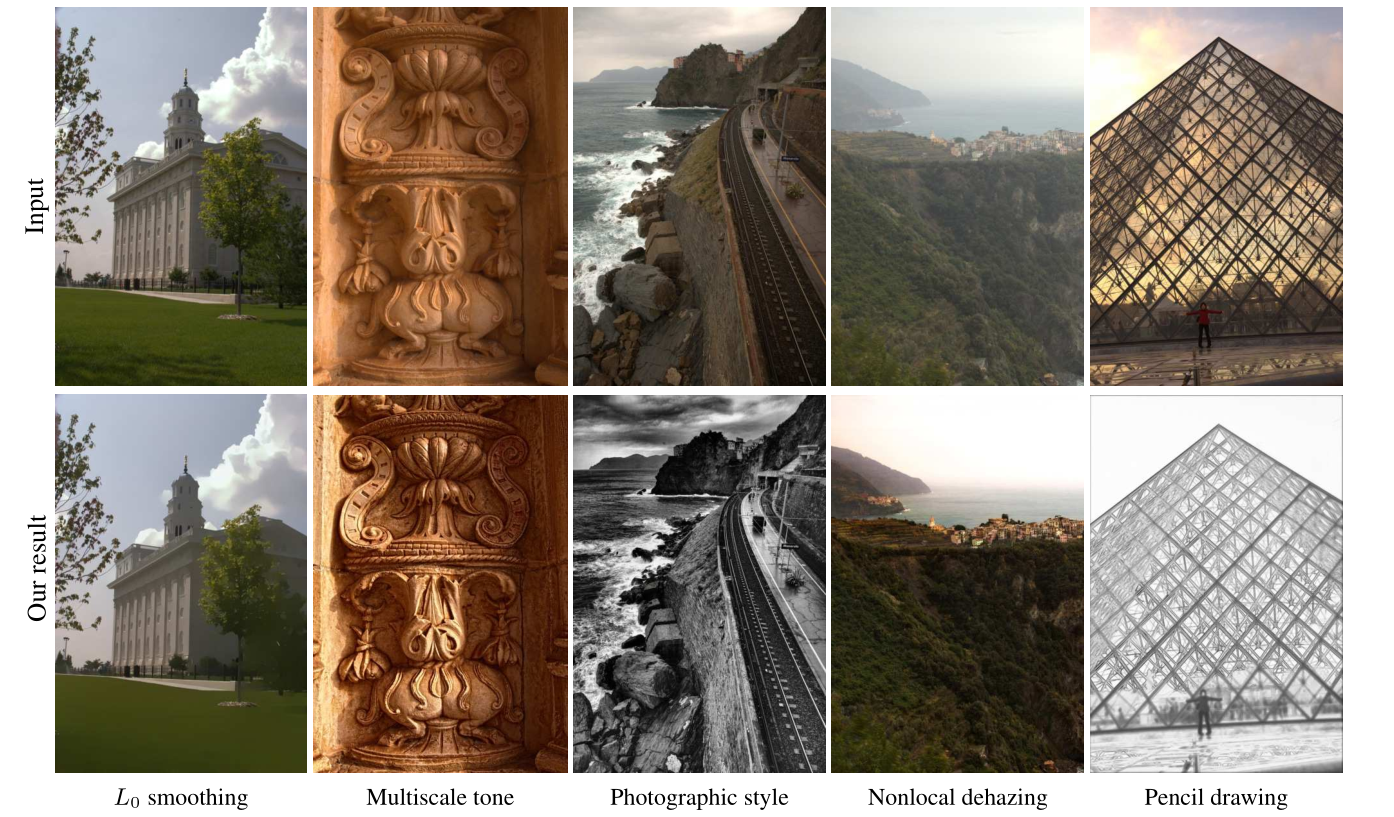
\includegraphics[width=1.0\textwidth]{1.png}
	\end{figure}	
\end{frame}




\begin{frame}{Algorithms}
	\begin{block}{ Context aggregation networks(CAN)}
		\begin{equation}
			\begin{split}
				\mathbf { L } _ { i } ^ { s } = \Phi \left( \Psi ^ { s } \left( b _ { i } ^ { s } + \sum _ { j } \mathbf { L } _ { j } ^ { s - 1 } * _ { r _ { s } } \mathbf { K } _ { i , j } ^ { s } \right) \right)
			\end{split}
		\end{equation}

		\begin{equation}
			\begin{split}
				\left( \mathbf { L } _ { j } ^ { s - 1 } * _ { r _ { s } } \mathbf { K } _ { i , j } ^ { s } \right) ( \mathbf { x } ) = \sum _ { \mathbf { a } + r _ { s } \mathbf { b } = \mathbf { x } } \mathbf { L } _ { j } ^ { s - 1 } ( \mathbf { a } ) \mathbf { K } _ { i , j } ^ { s } ( \mathbf { b } )
			\end{split}
		\end{equation}

		\begin{equation}
			\begin{split}
				\Psi ^ { s } ( x ) = \lambda _ { s } x + \mu _ { s } B N ( x )
			\end{split}
		\end{equation}

	\end{block}
\end{frame}

\begin{frame}{Algorithms}
	\begin{block}{ Image-space regression loss}
		\begin{equation}
			\begin{split}
				\ell ( \mathcal { K } , \mathcal { B } ) = \sum _ { i } \frac { 1 } { N _ { i } } \left\| \hat { f } \left( \mathbf { I } _ { i } ; \mathcal { K } , \mathcal { B } \right) - f \left( \mathbf { I } _ { i } \right) \right\| ^ { 2 }
			\end{split}
		\end{equation}
	\end{block}
\end{frame}

\begin{frame}{Experiments}
	\begin{block}{Qualitative results on images from the MIT-Adobe test set}
		\begin{figure}
			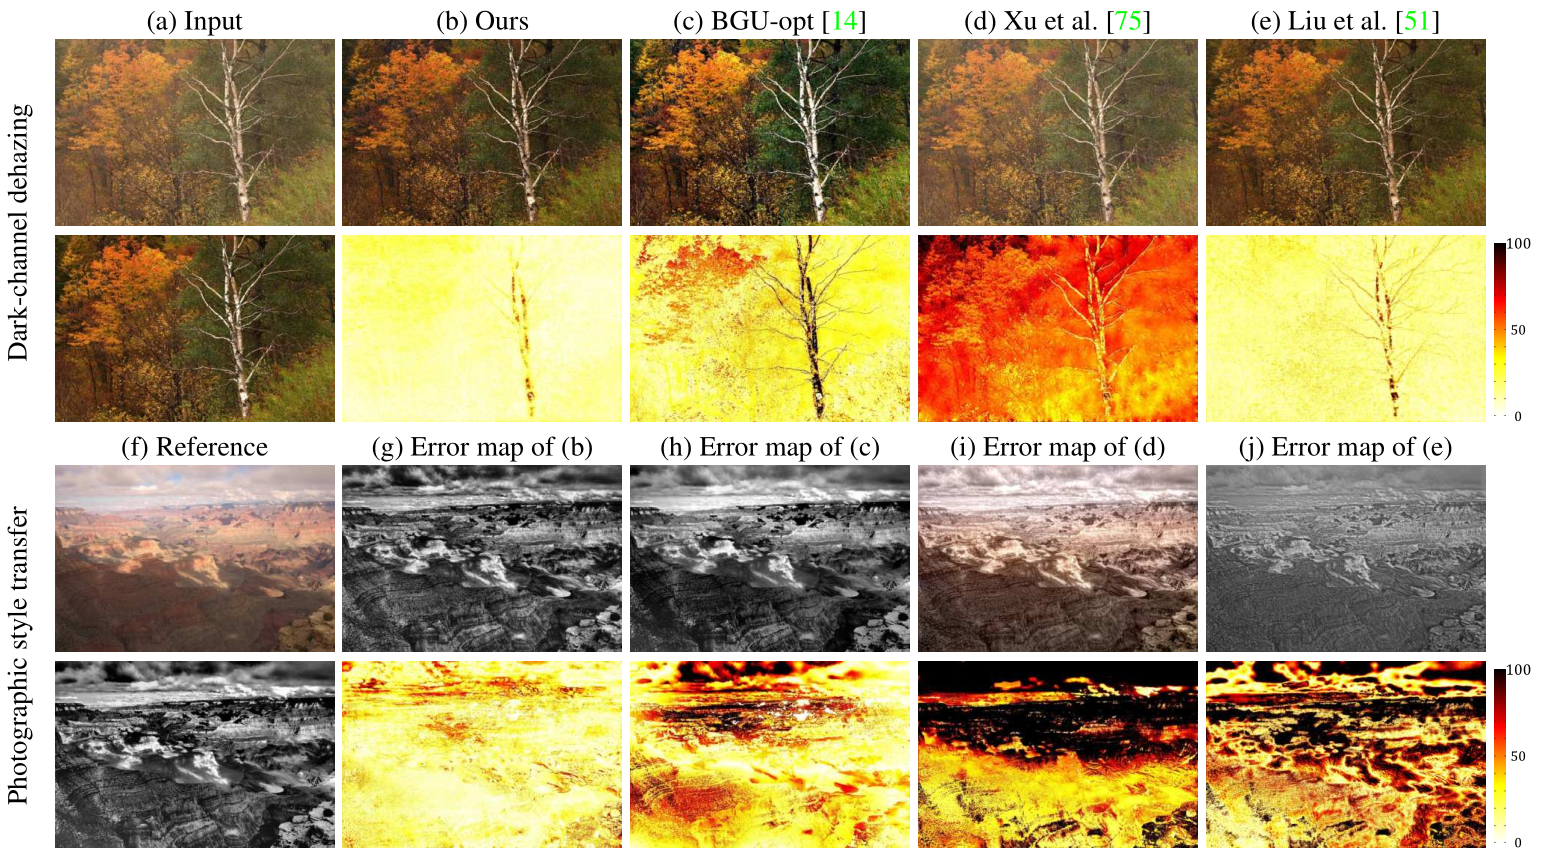
\includegraphics[width=1.0\textwidth]{2.png}
		\end{figure}
	\end{block}
\end{frame}



\begin{frame}{Further}
	\begin{block}{Ongoing Optimization}
		\begin{itemize}
			\item Parameterized operators. 
			\item One network to represent them all. 
			\item Video processing. 
		\end{itemize}
	\end{block}
\end{frame}


\begin{frame}{References}
	\begin{itemize}
		\item Qifeng Chen, Jia Xu, Vladlen Koltun \textit{Fast Image Processing with Fully-Convolutional Networks}
	
	\end{itemize}
\end{frame}




\end{document}
